\chapter{トレーディングアルゴリズム}
本章では,実際に使うトレーディングアルゴリズムを順に説明する.
\section{MACD}
ここではMACDを主に使うトレーディングアルゴリズムの説明をする.利確時の変数$tp$および損切り時の変数$sl$はアルゴリズム実行時,変更可能なパラメータである.

\subsection{MACDのみ}
MACDのみを使う場合のトレーディングアルゴリズムの説明をする.ここでは(B1)とする.
\begin{description}
\item[\textbf{Step~1~:}]MACDがシグナルを下から上へ突き抜けたときに翌日の始値で株を購入する.

\item[\textbf{Step~2~:}]以下の(2-1)~(2-2)のどちらかの条件が満たされれば売却する.
 \begin{description}
  \item[\textbf{(2-1):}]株の始値が購入した株価より$tp$%以上になった時点で売る.
  \item[\textbf{(2-2):}]株の始値が購入した株価より$sl$%以下になった時点で売る. 
 \end{description}
\item[\textbf{Step~3~:}]用意した株価データの最終日が来るまでStep 1からStep 3まで繰り返す.
\end{description}


図\ref{fig:macdonly}にMACDによる買いシグナルの例を示す.図\ref{fig:macdonly}の黒丸がMACDの買いシグナルで,その後$tp$%以上で売っている.
%%%%%%%%%%%%%%%%%

\subsection{MACDと60日移動平均線}
MACDと60日移動平均線を使う場合のトレーディングアルゴリズムを説明する.
長期の移動平均線の傾きが正の場合,株価も上昇する傾向にあるため,
MACDと組み合わせることで取引の勝率が上がると考えられ,それにより最終利益が増加すると想定している.
このアルゴリズムでは,60日平均線を長期線とする.ここでは(B2)とする.

\begin{figure}[t]
  \centering
  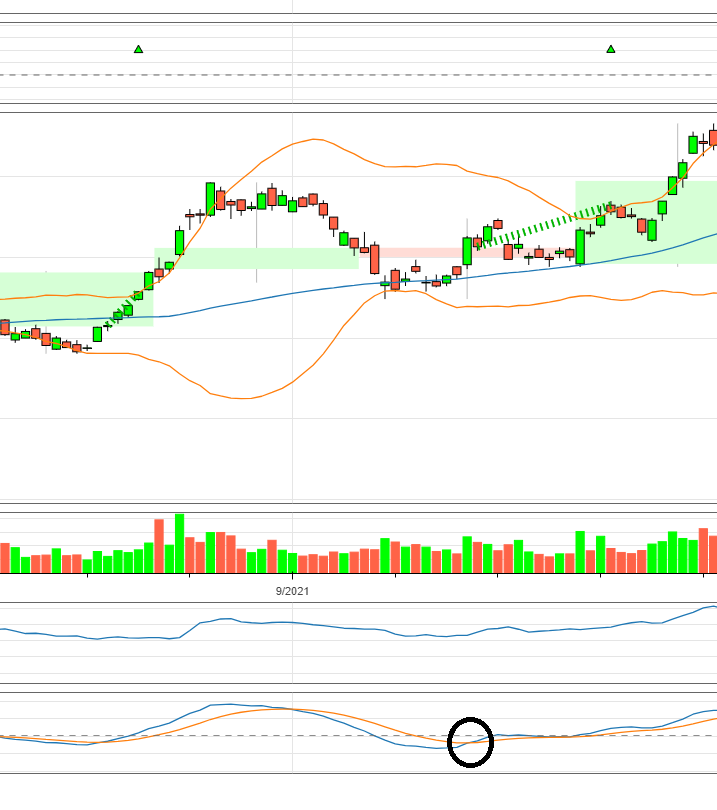
\includegraphics[width=110mm]{fig/macdonly.png}
  \caption{(B1)アルゴリズムの買いシグナル}
  \label{fig:macdonly}
 \end{figure}
\begin{description}
  \item[\textbf{Step~1~:}]以下の(1-1)~(1-2)のすべての条件が満たされれば翌日購入するする.
  \begin{description}
    \item[\textbf{(1-1):}]MACDがシグナルを下から上へ突き抜けたとき.
    \item[\textbf{(1-2):}]長期線の傾きが0以上のとき.
   \end{description}  
  
  \item[\textbf{Step~2~:}]以下の(2-1)~(2-2)のどちらかの条件が満たされれば売却する.
   \begin{description}
    \item[\textbf{(2-1):}]株の始値が購入した株価より$tp$%以上になった時点で売る.
    \item[\textbf{(2-2):}]株の始値が購入した株価より$sl$%以下になった時点で売る. 
   \end{description}
  \item[\textbf{Step~3~:}]用意した株価データの最終日が来るまでStep 1からStep 3まで繰り返す.
  \end{description}
  
   図\ref{fig:macdfma}にMACDと長期線よる買いシグナルの例を示す.図\ref{fig:macdfma}の黒丸がMACDの買いシグナルで,その時の長期線の傾きも0以上なので購入している.その後$tp$%以上で売っている.
   \begin{figure}[t]
    \centering
    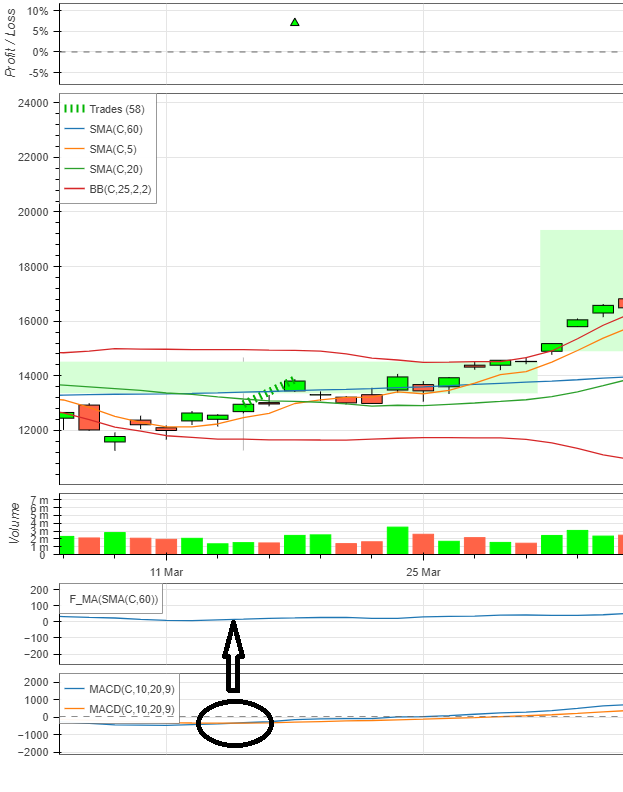
\includegraphics[width=110mm]{fig/macd_fma.png}
    \caption{(B2)アルゴリズムの買いシグナル}
    \label{fig:macdfma}
   \end{figure}

   %%%%%%%%%%%%%%%%%%

\subsection{MACDと日経株価平均}
MACDと日経平均株価を使う場合のトレーディングアルゴリズムを説明する.
日経株価平均は日本の主要な225銘柄を対象としており,日経株価平均が上昇しているということは市場全体が安定していると考えられ,
投資家の信頼があることを示唆している.つまり東証上位100社にもこの安定性が影響を及ぼすと考えられ,
それにより最終利益が増加すると想定している.
ここでは(B3)とする.
\begin{description}
  \item[\textbf{Step~1~:}]以下の(1-1)~(1-2)のすべての条件が満たされれば翌日購入するする.
  \begin{description}
    \item[\textbf{(1-1):}]注目する日のMACDがシグナルを下から上へ突き抜けたとき.
    \item[\textbf{(1-2):}]注目する日の日経平均株価の長期線の傾きが0以上のとき.
   \end{description}  
  
  
  \item[\textbf{Step~2~:}]以下の(2-1)~(2-2)のどちらかの条件が満たされれば売却する.
   \begin{description}
    \item[\textbf{(2-1):}]株の始値が購入した株価より$tp$%以上になった時点で売る.
    \item[\textbf{(2-2):}]株の始値が購入した株価より$sl$%以下になった時点で売る. 
   \end{description}
  \item[\textbf{Step~3~:}]用意した株価データの最終日が来るまでStep 1からStep 3まで繰り返す.
  \end{description}
  
   図\ref{fig:macdnk}にMACDと日経株価平均による買いシグナルの例を示す.図\ref{fig:macdnk}の黒丸がMACDの買いシグナルで,その時の日経株価平均の傾きも0以上なので購入している.その後$tp$%以上で売っている.


   %%%%%%%%%%%%%%%%%%

\subsection{MACDと日経株価平均と長期線}
MACDと日経平均株価と取引している株価データの長期線を使う場合のトレーディングアルゴリズムを説明する.
日経平均株価と取引している株価データの長期線を組み合わせることで,より勝率が上がると考えられ,
(B2),(B3)よりも最終利益が増加すると想定している.
ここでは二通りの方法を説明する.最初に説明するアルゴリズムを(B4),その後に説明するアルゴリズムを(B5)とする.


\begin{description}
    \item [\textbf{(B4):}]
    \item[\textbf{Step~1~:}]以下の(1-1)~(1-3)のすべての条件が満たされれば翌日購入するする.
    \begin{description}
      \item[\textbf{(1-1):}]注目する日のMACDがシグナルを下から上へ突き抜けたとき.
      \item[\textbf{(1-2):}]注目する日の日経平均株価の長期線の傾きが0以上のとき.
      \item[\textbf{(1-3):}]取引している株価データの長期線の傾きが0以上のとき. 
     \end{description}  
    
    
    \item[\textbf{Step~2~:}]以下の(2-1)~(2-2)のどちらかの条件が満たされれば売却する.
     \begin{description}
      \item[\textbf{(2-1):}]株の始値が購入した株価より$tp$%以上になった時点で売る.
      \item[\textbf{(2-2):}]株の始値が購入した株価より$sl$%以下になった時点で売る. 
     \end{description}
    \item[\textbf{Step~3~:}]用意した株価データの最終日が来るまでStep 1からStep 3まで繰り返す.

  \end{description}
    
     図\ref{fig:macdfmank}にMACD,長期線,日経株価平均による買いシグナルの例を示す.図\ref{fig:macdfmank}の黒丸がMACDの買いシグナルで,その上に表示されているその時の長期線の傾きと更に上の日経株価平均の傾きも0以上なので購入している.その後$tp$%以上で売っている.
  \begin{description}
    \begin{figure}[t]
      \centering
      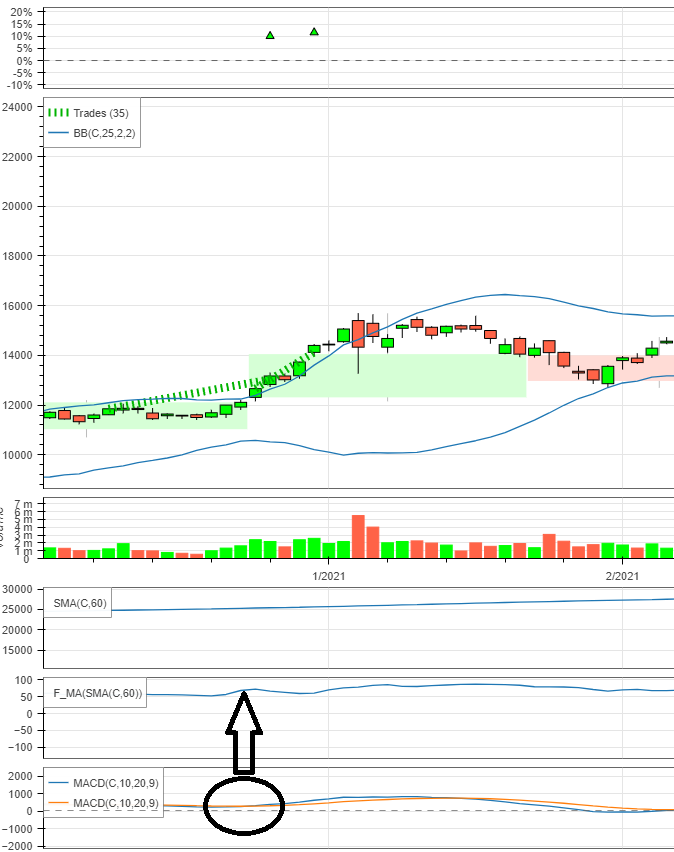
\includegraphics[width=110mm]{fig/macd_nk_paint.png}
      \caption{(B3)アルゴリズムの買いシグナル}
      \label{fig:macdnk}
     \end{figure}
    
    \item [\textbf{(B5):}]
    \item[\textbf{Step~1~:}]以下の(1-1)の条件と(1-2),(1-3)のどちらかの条件が満たされれば翌日購入するする.
    \begin{description}
      \item[\textbf{(1-1):}]注目する日のMACDがシグナルを下から上へ突き抜けたとき.
      \item[\textbf{(1-2):}]注目する日の日経平均株価の長期線の傾きが0以上のとき.
      \item[\textbf{(1-3):}]取引している株価データの長期線の傾きが0以上のとき. 

     \end{description}  
    
    
    \item[\textbf{Step~2~:}]以下の(2-1)~(2-2)のどちらかの条件が満たされれば売却する.
     \begin{description}
      \item[\textbf{(2-1):}]株の始値が購入した株価より$tp$%以上になった時点で売る.
      \item[\textbf{(2-2):}]株の始値が購入した株価より$sl$%以下になった時点で売る. 
     \end{description}
     \begin{figure}[H]
      \centering
      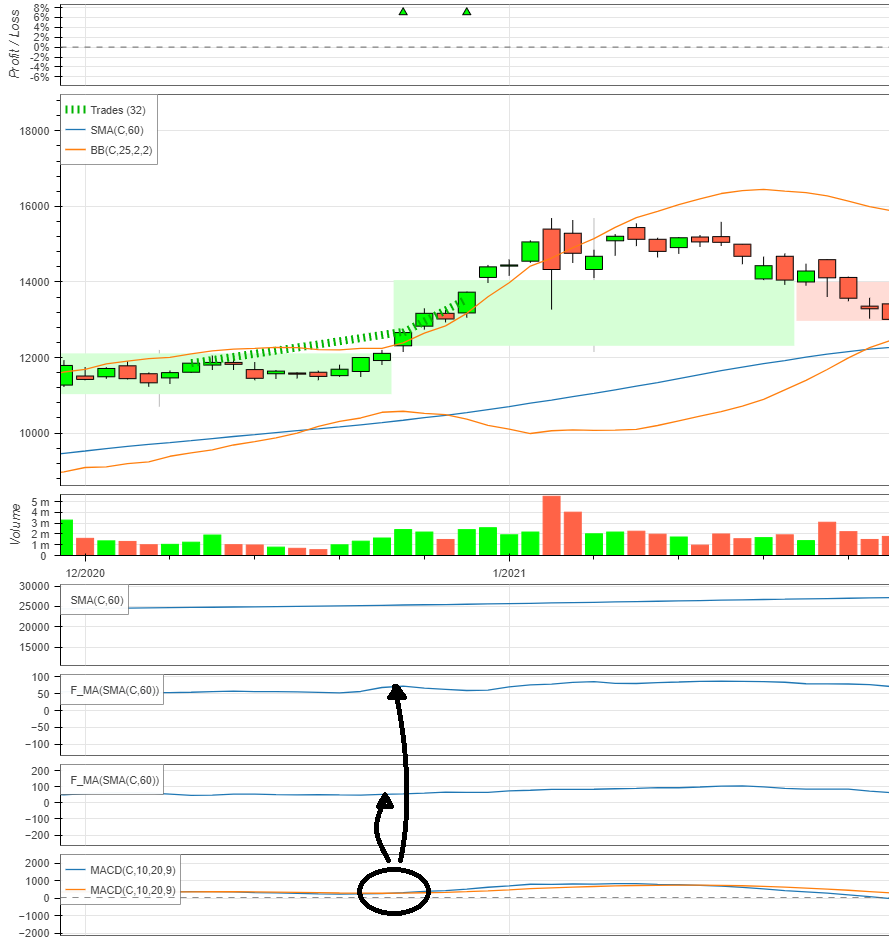
\includegraphics[width=110mm]{fig/macd_and_nk_and_fma_paint.png}
      \caption{(B4)アルゴリズムの買いシグナル}
      \label{fig:macdfmank}
     \end{figure}
    \item[\textbf{Step~3~:}]用意した株価データの最終日が来るまでStep 1からStep 3まで繰り返す.
\end{description}

  
 図\ref{fig:macdfma0nk},図\ref{fig:macdfmank0}に(B5)アルゴリズムの買いシグナルの例を示す.図\ref{fig:macdfma0nk}の黒丸がMACDの買いシグナルで,その時の赤丸の長期線の傾きは0以下だが青丸の日経株価平均の傾きが0以上なので購入している.その後$tp$%以上で売っている.
 また図\ref{fig:macdfmank0}の黒丸がMACDの買いシグナルで,その時の青丸の日経株価平均の傾きは0以下だが赤丸の長期線の傾きが0以上なので購入している.その後$tp$%以上で売っている.
%%%%%%%%%%%%%%%%%%
\section{BB}
ここではBBを主に使うトレーディングアルゴリズムの説明をする.利確時の変数$tp$および損切り時の変数$sl$はアルゴリズム実行時,変更可能なパラメータである.
\begin{figure}[t]
  \centering
  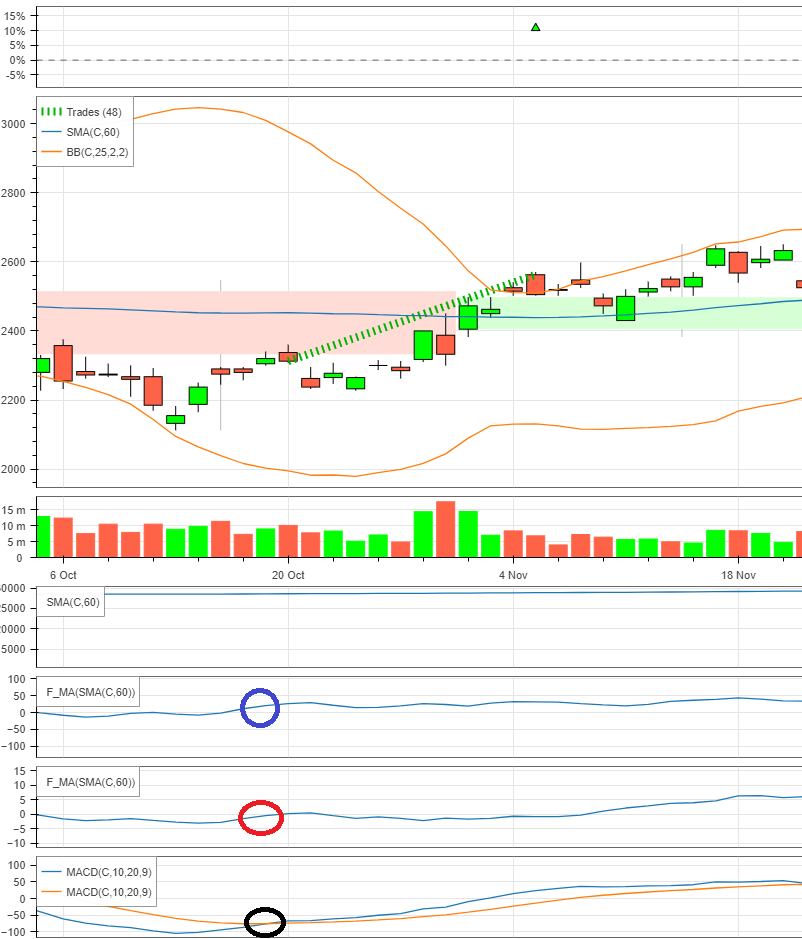
\includegraphics[width=110mm]{fig/macd_and_nk_or_fma0_6857_paint.png}
  \caption{(B5)アルゴリズムの(1-1)と(1-2)の買いシグナル}
  \label{fig:macdfma0nk}
 \end{figure}

 \begin{figure}[t]
  \centering
  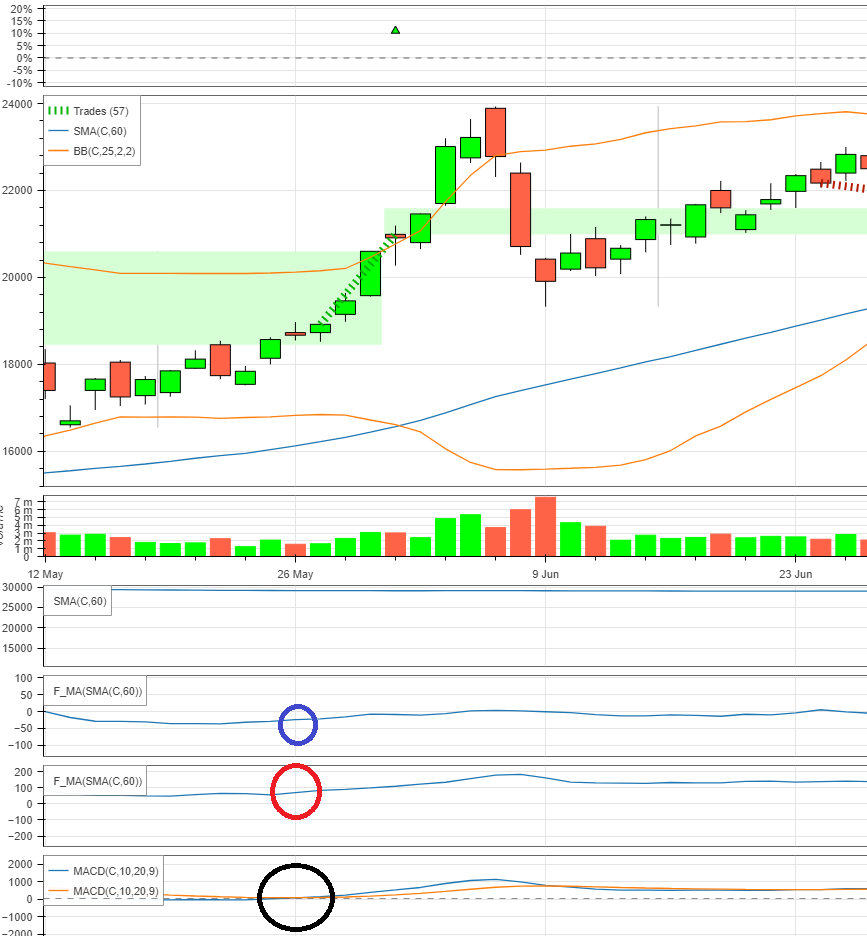
\includegraphics[width=110mm]{fig/macd_and_nk0_or_fma_paint.png}
  \caption{(B5)アルゴリズムの(1-1)と(1-3)の買いシグナル}
  \label{fig:macdfmank0}
 \end{figure}
\subsection{BBのみ}
BBのみを使う場合のトレーディングアルゴリズムの説明をする.ここでは(B6)とする.
\begin{description}
\item[\textbf{Step~1~:}]注目する日のローソクの終値が-2σのBBを上から下へ突き抜けたときに終値で株を購入する.

\item[\textbf{Step~2~:}]以下の(2-1)~(2-2)のどちらかの条件が満たされれば売却する.
 \begin{description}
  \item[\textbf{(2-1):}]株の始値が購入した株価より$tp$%以上になった時点で売る.
  \item[\textbf{(2-2):}]株の始値が購入した株価より$sl$%以下になった時点で売る. 
 \end{description}
\item[\textbf{Step~3~:}]用意した株価データの最終日が来るまでStep 1からStep 3まで繰り返す.
\end{description}

  
 図\ref{fig:bbonly}にBBによる買いシグナルの例を示す.図\ref{fig:bbonly}の黒丸がBBの買いシグナルで,その後$tp$%以上で売っている.
%%%%%%%%%%%%%%%%%%
\subsection{BBと60移動平均線}
BBと移動平均線を使う場合のトレーディングアルゴリズムの説明をする.60移動平均線を組み合わせる理由として(B2)と同じように,
取引の勝率が上がると考えられ,それにより最終利益が増加すると想定している.
ここでは(B7)とする.
\begin{description}
  \item[\textbf{Step~1~:}]以下の(1-1)~(1-2)のすべての条件が満たされれば終値で購入する.
  \begin{description}
    \item[\textbf{(1-1):}]注目する日のローソクの終値が-2σのBBを上から下へ突き抜けたときに終値で株を購入する.
    \item[\textbf{(1-2):}]長期線の傾きが0以上のとき.
   \end{description}  
   \begin{figure}[t]
    \centering
     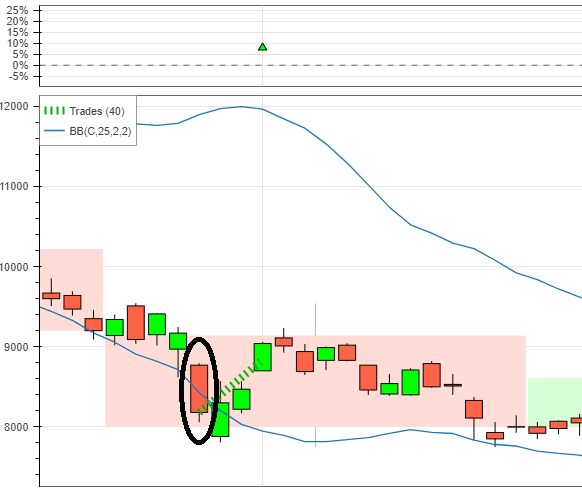
\includegraphics[width=110mm]{fig/bbonly_paint.png}
     \caption{(B6)アルゴリズムの買いシグナル}
     \label{fig:bbonly}
    \end{figure}
  \item[\textbf{Step~2~:}]以下の(2-1)~(2-2)のどちらかの条件が満たされれば売却する.
   \begin{description}
    \item[\textbf{(2-1):}]株の始値が購入した株価より$tp$%以上になった時点で売る.
    \item[\textbf{(2-2):}]株の始値が購入した株価より$sl$%以下になった時点で売る. 
   \end{description}
  \item[\textbf{Step~3~:}]用意した株価データの最終日が来るまでStep 1からStep 3まで繰り返す.
  \end{description}
  
   図\ref{fig:bbfma}にBBと長期線による買いシグナルの例を示す.図\ref{fig:bbfma}の黒丸がBBの買いシグナルで,その時の赤丸の長期線の傾きは0以上なので購入している.その後$tp$%以上で売っている.
%%%%%%%%%%%%%%%%%%
\subsection{BBと日経平均株価}
BBと日経平均株価を使う場合のトレーディングアルゴリズムの説明をする.日経平均株価を組み合わせる理由として(B3)と同じように,
取引の勝率が上がると考えられ,それにより最終利益が増加すると想定している.ここでは(B8)とする.
\begin{description}
  \item[\textbf{Step~1~:}]以下の(1-1)~(1-2)のすべての条件が満たされれば翌日購入するする.
  \begin{description}
    \item[\textbf{(1-1):}]注目する日のローソクの終値が-2σのBBを上から下へ突き抜けたときに終値で株を購入する.
    \begin{figure}[t]
      \centering
      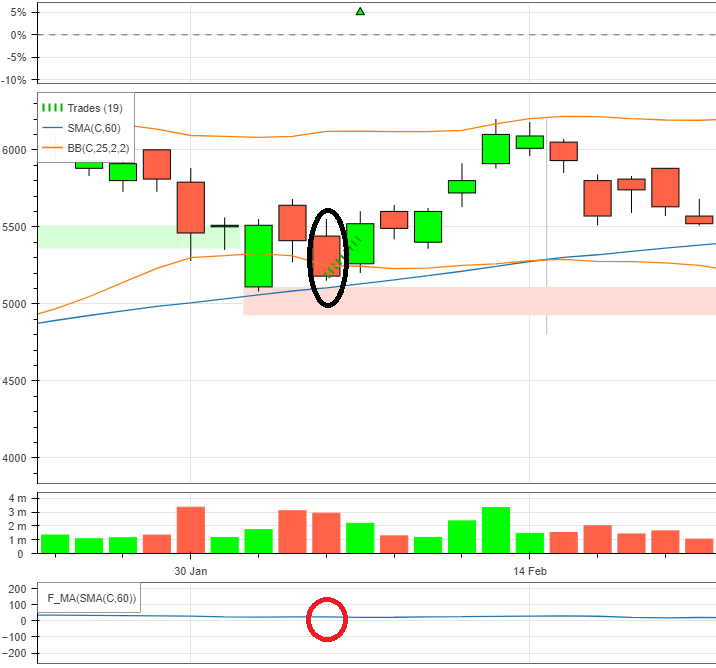
\includegraphics[width=110mm]{fig/bb_fma_paint.png}
      \caption{(B7)アルゴリズムの買いシグナル}
      \label{fig:bbfma}
     \end{figure}
    \item[\textbf{(1-2):}]注目する日の日経平均株価の長期線の傾きが0以上のとき.
   \end{description}  
  
  \item[\textbf{Step~2~:}]以下の(2-1)~(2-2)のどちらかの条件が満たされれば売却する.
   \begin{description}
    \item[\textbf{(2-1):}]株の始値が購入した株価より$tp$%以上になった時点で売る.
    \item[\textbf{(2-2):}]株の始値が購入した株価より$sl$%以下になった時点で売る. 
   \end{description}
  \item[\textbf{Step~3~:}]用意した株価データの最終日が来るまでStep 1からStep 3まで繰り返す.
  \end{description}
  
   図\ref{fig:bbnk}にBBと日経株価平均による買いシグナルの例を示す.図\ref{fig:bbnk}の黒丸がBBの買いシグナルで,その時の赤丸の日経株価平均の傾きは0以上なので購入している.その後$tp$%以上で売っている.
%%%%%%%%%%%%%%%%%%

\subsection{BBと日経株価平均と長期線}
BBと日経平均株価と取引している株価データの長期線を使う場合のトレーディングアルゴリズムを説明する. (B4),(B5)同じように,取引の勝率が上がると考
えられ,それにより最終利益が増加すると想定している.
ここでは二通りの方法を説明する.最初に説明するアルゴリズムを(B9),その後に説明するアルゴリズムを(B10)とする.
\begin{figure}[t]
  \centering
  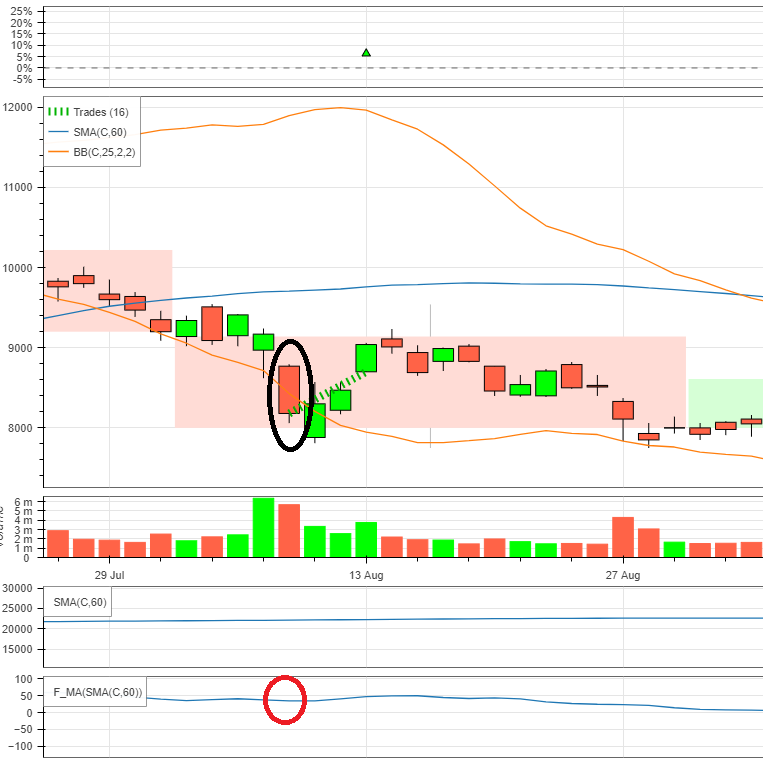
\includegraphics[width=110mm]{fig/bb_nk_paint.png}
  \caption{(B8)アルゴリズムの買いシグナル}
  \label{fig:bbnk}
 \end{figure}
\begin{description}
  \item[\textbf{(B9):}]
    \item[\textbf{Step~1~:}]以下の(1-1)~(1-3)のすべての条件が満たされれば翌日購入するする.
    \begin{description}
      \item[\textbf{(1-1):}]注目する日のローソクの終値が-2σのBBを上から下へ突き抜けたときに終値で株を購入する.
      \item[\textbf{(1-2):}]注目する日の日経平均株価の長期線の傾きが0以上のとき.
      \item[\textbf{(1-3):}]取引している株価データの長期線の傾きが0以上のとき. 
     
    \item[\textbf{Step~2~:}]以下の(2-1)~(2-2)のどちらかの条件が満たされれば売却する.
     \begin{description}
      \item[\textbf{(2-1):}]株の始値が購入した株価より$tp$%以上になった時点で売る.
      \item[\textbf{(2-2):}]株の始値が購入した株価より$sl$%以下になった時点で売る. 
     \end{description}
    \item[\textbf{Step~3~:}]用意した株価データの最終日が来るまでStep 1からStep 3まで繰り返す.
    \end{description}
  \end{description}  
 
   
  図\ref{fig:bbnkfma}にBB,長期線,日経株価平均による買いシグナルの例を示す.図\ref{fig:bbnkfma}の黒丸がBBの買いシグナルで,その時の長期線の傾きと日経株価平均の傾きも0以上なので購入している.その後$tp$%以上で売っている.

  \begin{description}
    \item[\textbf{(B10):}]
    \item[\textbf{Step~1~:}]以下の(1-1)の条件と(1-2),(1-3)のどちらかの条件が満たされれば終値で購入する.
    \begin{description}
      \item[\textbf{c:}]注目する日のローソクの終値が-2σのBBを上から下へ突き抜けたときに終値で株を購入する.
      \item[\textbf{(1-2):}]注目する日の日経平均株価の長期線の傾きが0以上のとき.
      \item[\textbf{(1-3):}]取引している株価データの長期線の傾きが0以上のとき. 

     \end{description}  
    
    
    \item[\textbf{Step~2~:}]以下の(2-1)~(2-2)のどちらかの条件が満たされれば売却する.
     \begin{description}
      \item[\textbf{(2-1):}]株の始値が購入した株価より$tp$%以上になった時点で売る.
      \item[\textbf{(2-2):}]株の始値が購入した株価より$sl$%以下になった時点で売る. 
     \end{description}
    \item[\textbf{Step~3~:}]用意した株価データの最終日が来るまでStep 1からStep 3まで繰り返す.
    \end{description}
    
     図\ref{fig:bbnkfma0},及び,図\ref{fig:bbnk0fma}に,(B10)アルゴリズムによる買いシグナルの例を示す.図\ref{fig:bbnkfma0}の黒丸がBBの買いシグナルで,その時の赤丸の長期線の傾きは0以下だが青丸の日経株価平均の傾きが0以上なので購入している.その後$tp$%以上で売っている.
 また図\ref{fig:bbnk0fma}の黒丸がBBの買いシグナルで,その時の青丸の日経株価平均の傾きは0以下だが赤丸の長期線の傾きが0以上なので購入している.その後$tp$%以上で売っている.
%%%%%%%%%%%%%%%%%%%%%%%%%%%%%%%%%%%%%%%%%%%%%%%%%%%%%%%%%%%%%%%
\section{MACDとBB}
ここではMACDとBBを主に使うトレーディングアルゴリズムの説明をする.利確時の変数$tp$および損切り時の変数$sl$はアルゴリズム実行時,変更可能なパラメータである.
\subsection{MACDとBB}
MACDとBBを使う場合のトレーディングアルゴリズムを説明する.2つを組み合わせることでより良い効果が得られるのではないかと想定している.ここでは(B11)とする.
\begin{figure}[H]
  \centering
    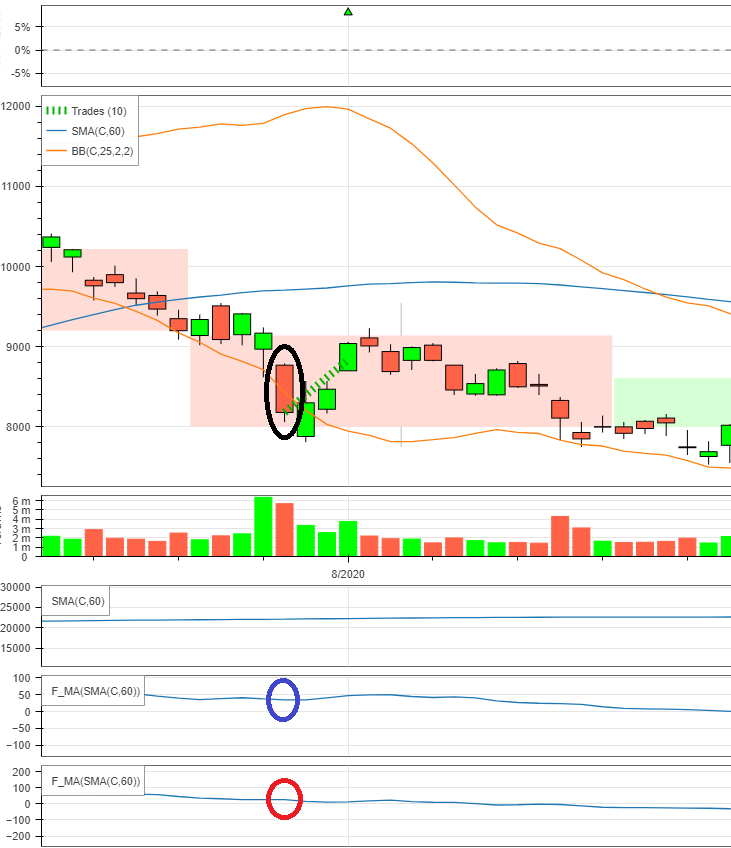
\includegraphics[width=110mm]{fig/bb_and_nk_and_fma_paint.png}
    \caption{(B9)アルゴリズムの買いシグナル}
    \label{fig:bbnkfma}
   \end{figure}

   


   \begin{figure}[H]
    \centering
    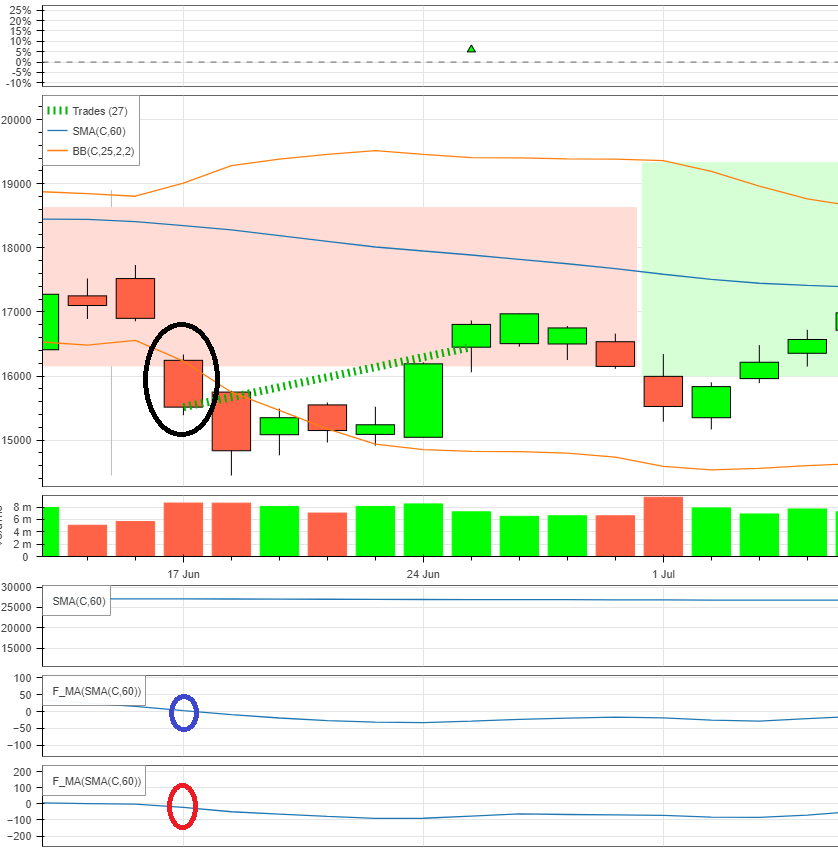
\includegraphics[width=110mm]{fig/bb_and_nk_or_fma0_paint.png}
    \caption{(B10)アルゴリズムの(1-1)と(1-2)の買いシグナル}
    \label{fig:bbnkfma0}
   \end{figure}

   \begin{figure}[H]
    \centering
    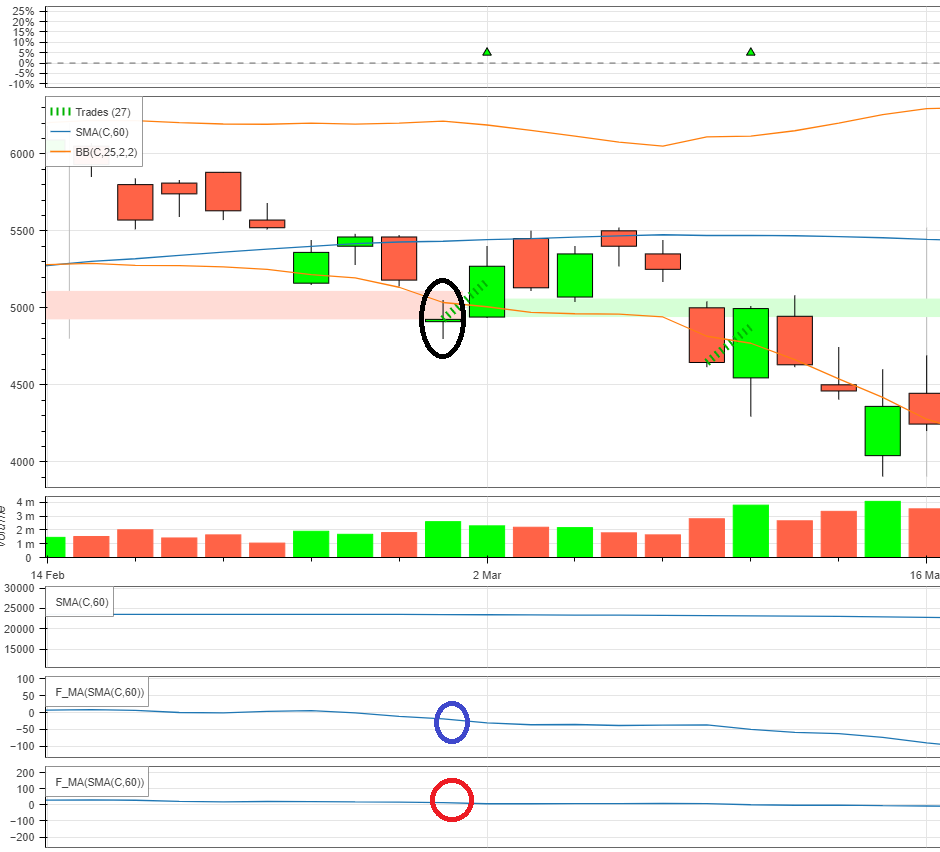
\includegraphics[width=110mm]{fig/bb_and_nk0_or_fma_paint.png}
    \caption{(B10)アルゴリズムの(1-1)と(1-3)の買いシグナル}
    \label{fig:bbnk0fma}
   \end{figure}
\begin{description}
  \item[\textbf{Step~1~:}]以下の(1-1)~(1-2)のどちらかの条件が満たされれば購入する.
  \begin{description}
    \item[\textbf{(1-1):}]MACDがシグナルを下から上へ突き抜けたときに翌日の始値で株を購入する.
    \item[\textbf{(1-2):}]注目する日のローソクの終値が-2σのBBを上から下へ突き抜けたときに終値で株を購入する.
   \end{description}  
  
  \item[\textbf{Step~2~:}]以下の(2-1)~(2-2)のどちらかの条件が満たされれば売却する.
   \begin{description}
    \item[\textbf{(2-1):}]株の始値が購入した株価より$tp$%以上になった時点で売る.
    \item[\textbf{(2-2):}]株の始値が購入した株価より$sl$%以下になった時点で売る. 
   \end{description}
  \item[\textbf{Step~3~:}]用意した株価データの最終日が来るまでStep 1からStep 3まで繰り返す.
  \end{description}
  


図\ref{fig:bb0macd},図\ref{fig:bbmacd0}にMACDとBよる買いシグナルの例を示す.図\ref{fig:bb0macd}の黒丸のBBはなにも起きていないが,赤丸がMACDの買いシグナルになっているので購入している.その後$tp$%以上で売っている.また,
図\ref{fig:bbmacd0}の赤丸のMACDはなにも起きていないが,黒丸がBBの買いシグナルになっているので購入している.その後$tp$%以上で売っている.
  %%%%%%%%%%%%%%%%
  \begin{figure}[H]
    \centering
    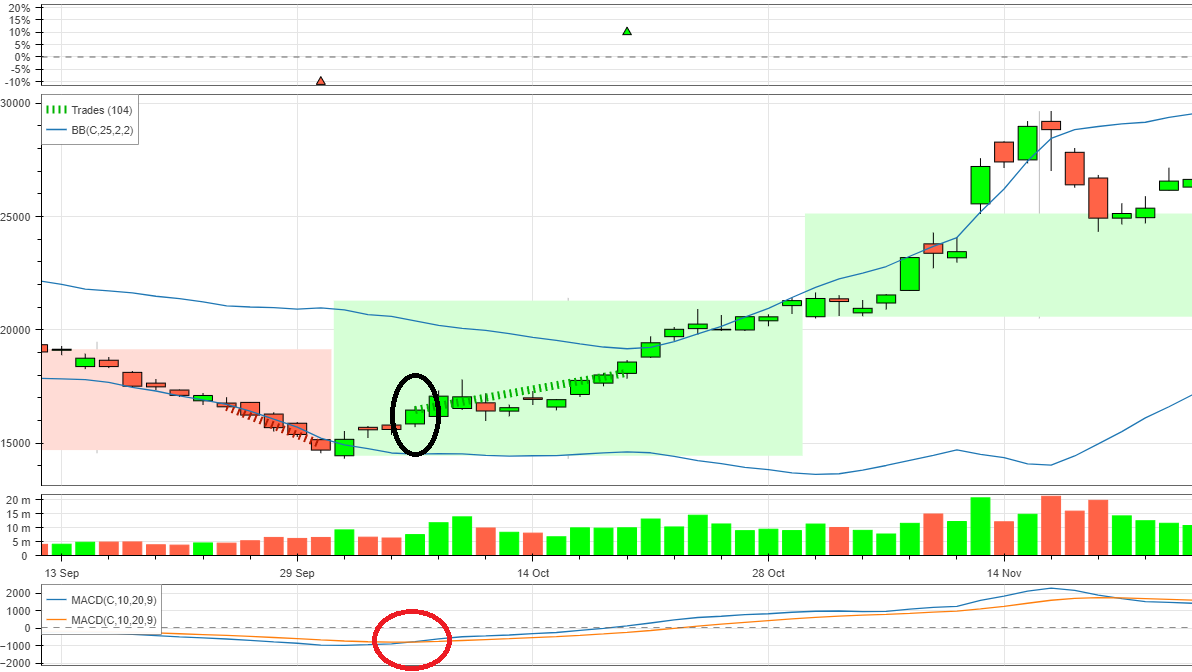
\includegraphics[width=110mm]{fig/bb0_or_macd_paint.png}
    \caption{(B11)アルゴリズムの(1-2)の買いシグナル}
    \label{fig:bb0macd}
   \end{figure}

  \begin{figure}[H]
    \centering
    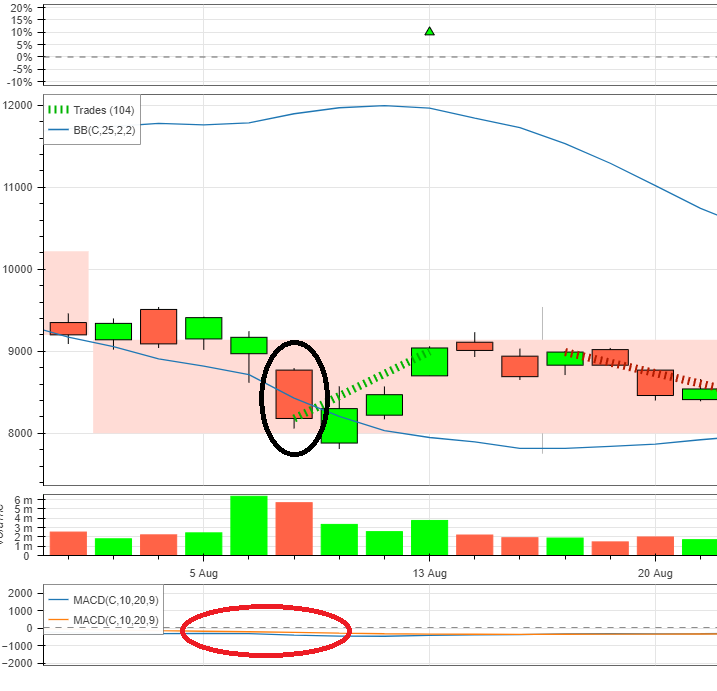
\includegraphics[width=110mm]{fig/bb_or_macd0_paint.png}
    \caption{(B11)アルゴリズムの(1-1)の買いシグナル}
    \label{fig:bbmacd0}
   \end{figure}
\subsection{MACDとBBと60日移動平均線}
MACDとBBと長期線を使う場合のトレーディングアルゴリズムを説明する.ここでは二通りの方法を説明する.(B11)に移動平均線を加えることで安定して勝率が上がるのではないかと想定している.ここでは最初に説明するアルゴリズムを(B12),その後に説明するアルゴリズムを(B13)とする.

   \begin{description}
    \item[\textbf{(B12):}]
    \item[\textbf{Step~1~:}]以下の(1-1)~(1-2)のどちらかと(1-3)の条件が満たされれば翌日購入するする.
    \begin{description}
      \item[\textbf{(1-1):}]注目する日のMACDがシグナルを下から上へ突き抜けたとき.
      \item[\textbf{(1-2):}]注目する日のローソクの終値が-2σのBBを上から下へ突き抜けたときに翌日の始値で株を購入する.
      \item[\textbf{(1-3):}]取引している株価データの長期線の傾きが0以上のとき. 
     \end{description}  
    
    
    \item[\textbf{Step~2~:}]以下の(2-1)~(2-2)のどちらかの条件が満たされれば売却する.
     \begin{description}
      \item[\textbf{(2-1):}]株の始値が購入した株価より$tp$%以上になった時点で売る.
      \item[\textbf{(2-2):}]株の始値が購入した株価より$sl$%以下になった時点で売る. 
     \end{description}
    \item[\textbf{Step~3~:}]用意した株価データの最終日が来るまでStep 1からStep 3まで繰り返す.
    \end{description}

    

     図\ref{fig:bb0ormacdfma},図\ref{fig:bbormacd0fma}にB12アルゴリズムの買いシグナルの例を示す.図\ref{fig:bb0ormacdfma}の青丸のBBはなにも起きていないが,黒丸がMACDの買いシグナルになっているのと,赤丸の長期線の傾きも0以上なので購入している.その後$tp$%以上で売っている.また,
     図\ref{fig:bbormacd0fma}の青丸のMACDはなにも起きていないが,黒丸がBBの買いシグナルになっているのと,赤丸の長期線の傾きも0以上なので購入している.その後$tp$%以上で売っている.
 
     \begin{description}
    \item[\textbf{(B13):}]
    \item[\textbf{Step~1~:}]以下の(1-1)の条件または(1-2),(1-3)のすべての条件が満たされれば翌日購入する.
    \begin{description}
      \item[\textbf{(1-1):}]注目する日のMACDがシグナルを下から上へ突き抜けたとき.
      \item[\textbf{(1-2):}]注目する日のローソクの終値が-2σのBBを上から下へ突き抜けたときに翌日の始値で株を購入する.
      \item[\textbf{(1-3):}]取引している株価データの長期線の傾きが0以上のとき. 

     \end{description}  
     \begin{figure}[H]
      \centering
      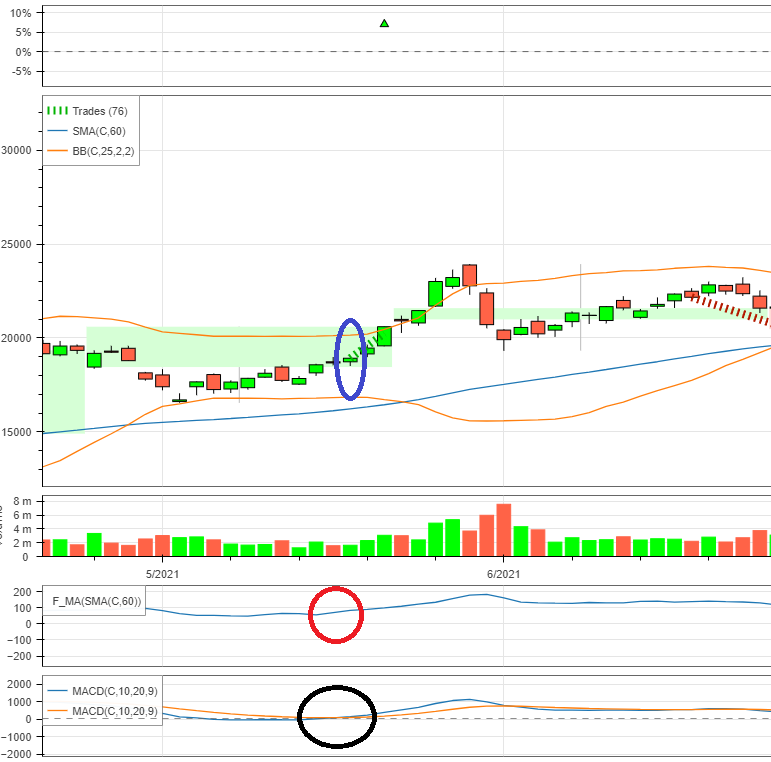
\includegraphics[width=110mm]{fig/macdorbb0_and_fma_paint.png}
      \caption{(B12)アルゴリズムの(1-1)と(1-3)の買いシグナル}
      \label{fig:bb0ormacdfma}
     \end{figure}
  
     \begin{figure}[H]
      \centering
      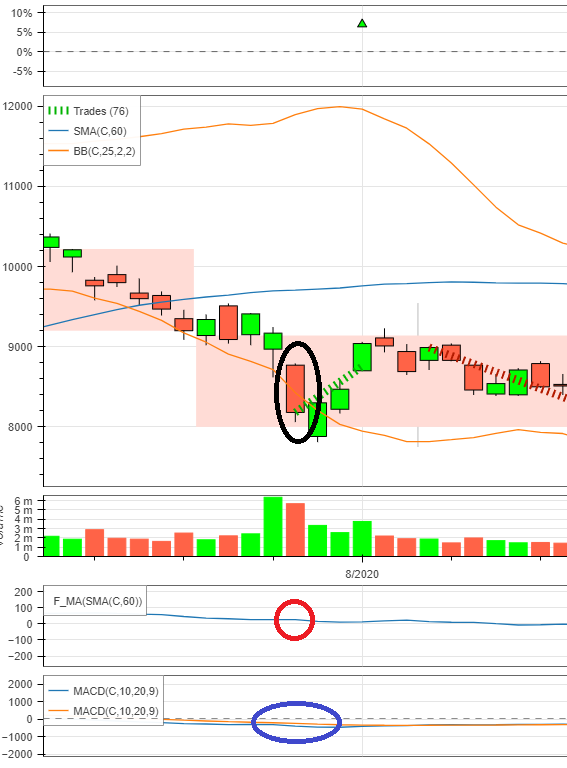
\includegraphics[width=110mm]{fig/macd0orbb_and_fma_paint.png}
      \caption{(B12)アルゴリズムの(1-2)と(1-3)の買いシグナル}
      \label{fig:bbormacd0fma}
     \end{figure}
    
    \item[\textbf{Step~2~:}]以下の(2-1)~(2-2)のどちらかの条件が満たされれば売却する.
     \begin{description}
      \item[\textbf{(2-1):}]株の始値が購入した株価より$tp$%以上になった時点で売る.
      \item[\textbf{(2-2):}]株の始値が購入した株価より$sl$%以下になった時点で売る. 
     \end{description}
    \item[\textbf{Step~3~:}]用意した株価データの最終日が来るまでStep 1からStep 3まで繰り返す.
    \end{description}

    
     図\ref{fig:bbfma0ormacd},図\ref{fig:bbfmaormacd0}に(B13)の買いシグナルの例を示す.図\ref{fig:bbfma0ormacd}の黒丸がMACDの買いシグナルになっているのと,赤丸の長期線の傾きも0以上だが青丸のBBはなにも起きていため,MACDの買いシグナルのみで購入している.その後$tp$%以上で売っている.また,
     図\ref{fig:bbfmaormacd0}の青丸のMACDはなにも起きていないが,黒丸がBBの買いシグナルになっているのと,赤丸の長期線の傾きも0以上なので購入している.その後$tp$%以上で売っている.







     
 

 




 


  



   

   \begin{figure}[H]
    \centering
    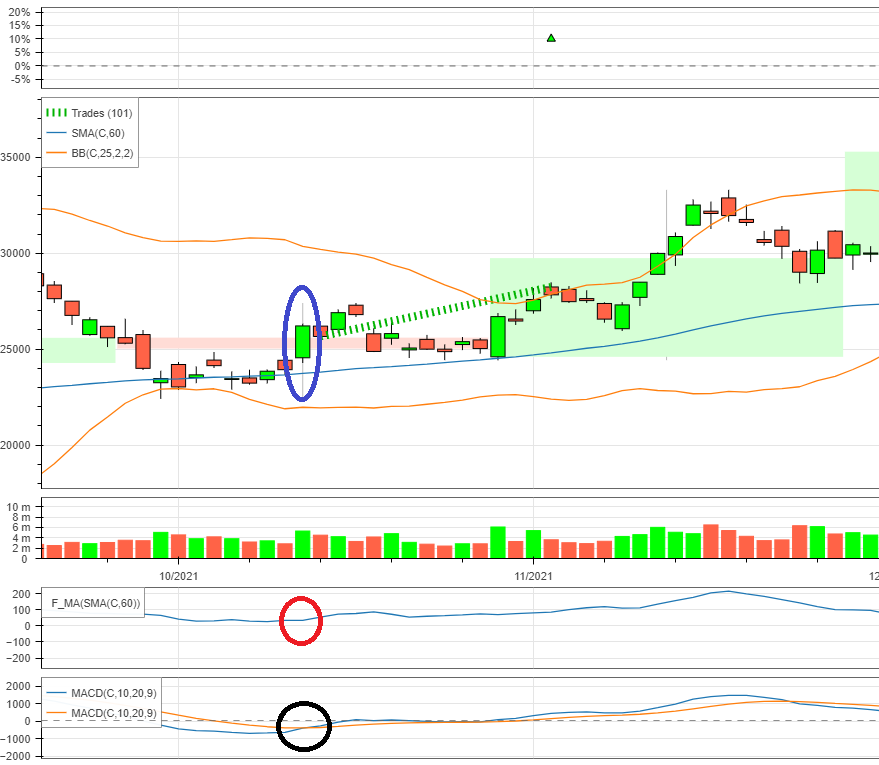
\includegraphics[width=110mm]{fig/bbandfma0_or_macd_paint.png}
    \caption{(B13)アルゴリズムの(1-1)の買いシグナル}
    \label{fig:bbfma0ormacd}
   \end{figure}

   \begin{figure}[H]
    \centering
    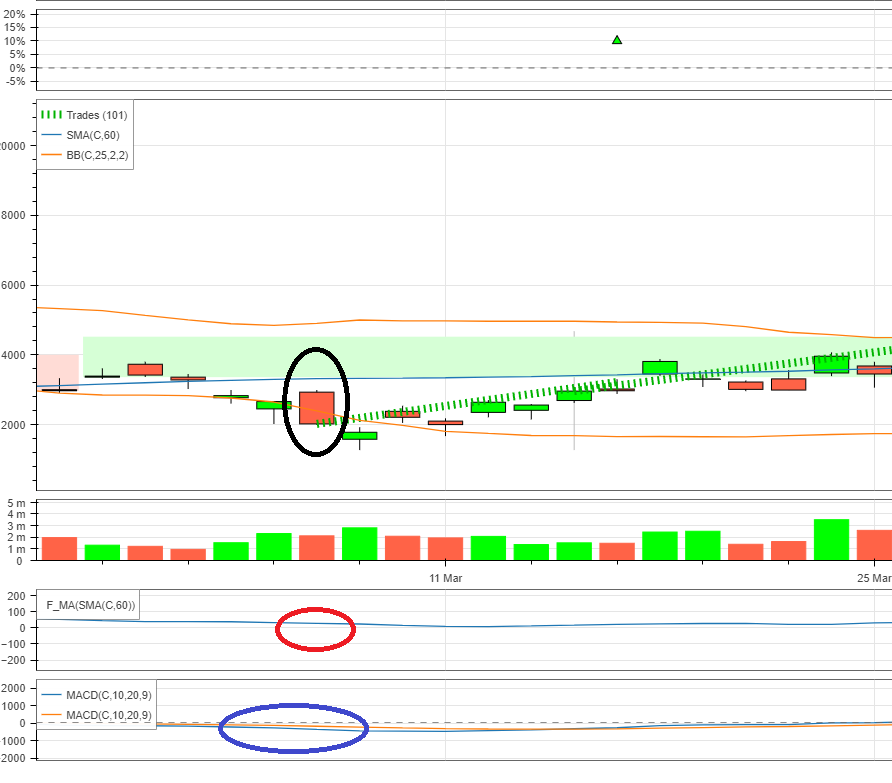
\includegraphics[width=110mm]{fig/bbandfma_or_macd0_paint.png}
    \caption{(B13)アルゴリズムの(1-2)と(1-3)の買いシグナル}
    \label{fig:bbfmaormacd0}
   \end{figure}
     \newpage